\documentclass[letterpaper]{article}

\usepackage{natbib,alifeconf}  %% The order is important
\usepackage{url,hyperref,cleveref}
\usepackage{booktabs}
\usepackage{multirow}
\usepackage{graphicx}
\usepackage{xcolor}

\newcommand\blfootnote[1]{%
  \begingroup
  \renewcommand\thefootnote{}\footnote{#1}%
  \addtocounter{footnote}{-1}%
  \endgroup
}

\title{CheeseBench: Evaluating Large Language Models\\on Rodent Behavioral Neuroscience Paradigms}

\author{
    Zacharie Bugaud$^{1}$ \\
    \mbox{}\\
    $^1$Astera Institute \\
    zacharie@astera.org
}

\begin{document}

\maketitle

\begin{abstract}
We introduce \textsc{CheeseBench}, a benchmark that evaluates large language models (LLMs) on nine classical behavioral neuroscience paradigms (Morris water maze, Barnes maze, T-maze, radial arm maze, star maze, operant chamber, shuttle box, conditioned place preference, and delayed non-match to sample), spanning six cognitive dimensions.
Each task is grounded in peer-reviewed rodent protocols with approximate animal baselines.
The agent receives a unified system prompt with no task-specific instructions and must discover goals purely from ASCII text observations and reward signals, much like a rodent placed into an unfamiliar apparatus.
We evaluate six open-weight LLMs (3B to 72B parameters) on text-based ASCII renderings and compare against both a random baseline and a graph-based reinforcement learning agent.
Our best model (Qwen2.5-VL-7B) reaches 52.6\% average success on ASCII input, compared to 32.1\% for random agents and 78.9\% for approximate rodent baselines.
We find that (1)~scaling beyond 7B yields diminishing returns, (2)~longer context history degrades performance, (3)~chain-of-thought prompting hurts rather than helps, and (4)~a vision-language architecture provides an advantage at 7B but hurts at 32B.
Because the same model's performance ranges from 20\% to 57\% depending on interface parameters alone, these results characterize the agent-plus-interface system, not the model in isolation.
Under this unified zero-shot ASCII protocol, current open-weight LLM agents remain well below approximate rodent reference values, particularly on tasks requiring spatial navigation and within-trial state tracking.
\end{abstract}

Submission type: \textbf{Full Paper}
\blfootnote{\textcopyright~2026 Zacharie Bugaud. Published under a Creative Commons Attribution 4.0 International (CC BY 4.0) license.}


\section{Introduction}

Large language models (LLMs) now perform well on question answering, reasoning, and multimodal benchmarks \citep{liu2024visual,team2024gemini}.
But these benchmarks primarily test declarative knowledge: recognizing objects, answering factual questions, or following explicit instructions.
A different kind of intelligence is procedural learning, i.e., discovering goals through trial and error, building spatial representations, and adapting behavior based on reward feedback.
This is what behavioral neuroscience has measured in laboratory animals for over a century.

Rodent behavioral paradigms provide standardized, reproducible assays of cognitive function \citep{vorhees2006morris,shoji2012t}.
Tasks like the Morris water maze and radial arm maze probe specific neural circuits: hippocampal place cells for spatial learning \citep{okeefe1971hippocampus}, working memory \citep{olton1976spatial}, and instrumental conditioning \citep{skinner1938behavior}.
These paradigms make natural AI benchmarks because they are (i)~mechanistically well-understood, (ii)~come with quantitative animal baselines from decades of research, and (iii)~test capabilities that current LLM benchmarks largely ignore.

We present \textsc{CheeseBench}, a benchmark suite of nine environments spanning six cognitive dimensions (\Cref{tab:environments}).
Each environment implements a published rodent protocol as a gridworld rendered as ASCII text (\Cref{fig:environments}).
Three rendering modes are available (ASCII top-down, egocentric, and pseudo-3D first-person), with ASCII top-down used as the default for all experiments.
The agent receives a single unified system prompt identical across all tasks, with no task-specific instructions, hints, or reward shaping.
It must discover the goal, form a strategy, and improve over repeated trials, just as a rodent placed in an unfamiliar apparatus would.
The primary goal of CheeseBench is to evaluate how well current LLM agent configurations perform on procedural discovery under a unified blind protocol; the rodent data serve as approximate biological reference points rather than strict competitive baselines.

Our contributions are:
\begin{enumerate}
    \item A benchmark suite of 9 behavioral neuroscience paradigms with approximate rodent reference values, covering 6 cognitive dimensions.
    \item A systematic evaluation of 6 open-weight LLMs (3B to 72B) on ASCII text input, characterizing the agent-plus-interface system and showing that even the best configuration falls well short of approximate rodent reference values.
    \item Ablation studies showing that longer context hurts, chain-of-thought hurts, and the advantage of visual input over ASCII text is scale-dependent.
\end{enumerate}


\section{Related Work}

\paragraph{LLM and VLM Benchmarks.}
Standard VLM benchmarks such as VQA \citep{antol2015vqa}, MMLU \citep{hendrycks2021measuring}, and MathVista \citep{lu2024mathvista} primarily assess declarative reasoning.
Interactive benchmarks like ALFWorld \citep{shridhar2021alfworld} and WebArena \citep{zhou2024webarena} test procedural capabilities but use task-specific instructions and structured feedback.
\textsc{CheeseBench} uses a unified blind protocol with only scalar reward feedback.

\paragraph{Animal Cognition as AI Benchmark.}
The Animal-AI Testbed \citep{crosby2020animal} pioneered evaluating AI on animal cognition tests but focused on 3D physics (Unity engine) without direct rodent protocol fidelity.
Concurrent work has proposed bird cognition \citep{voudouris2023direct} and primate tests for LLMs.
Our work differs in that each environment maps to a specific published rodent protocol with approximate baselines derived from the peer-reviewed literature.

\paragraph{Cognitive Profiling of LLMs.}
Recent work has adapted human psychological batteries (Theory of Mind, analogical reasoning) to test LLMs \citep{kosinski2023theory,webb2023emergent}.
We complement this by using the nonverbal, reward-driven paradigms standard in comparative psychology.


\section{CheeseBench Benchmark}

\subsection{Design Principles}

\textsc{CheeseBench} follows four principles inspired by how behavioral neuroscience studies are conducted:

\begin{enumerate}
\item \textbf{Unified protocol.} A single system prompt for all nine tasks. No task-specific instructions, reward explanations, or goal descriptions. The agent must discover task structure through exploration and reward feedback.
\item \textbf{Approximate biological references.} Each environment corresponds to a real rodent experiment. We derive reference success rates from published learning curves by mapping the original outcome metric to our binary criterion (see the Rodent Baseline Construction appendix). These are constructed reference anchors, not direct competitive baselines.
\item \textbf{Cognitive taxonomy.} Environments span six cognitive dimensions, enabling profiling across distinct neural substrates.
\item \textbf{Multi-action episodes.} The agent outputs up to $k$ actions per API call along with free-text ``learnings'' that serve as an explicit working memory, mimicking the episodic structure of animal experiments.
\end{enumerate}

\subsection{Environments}

\Cref{tab:environments} lists all nine paradigms.  We briefly describe representative tasks:

\paragraph{Morris Water Maze (MWM).}
A circular arena with a hidden escape platform. The agent uses distal landmarks for allocentric navigation. Rodents typically reach asymptotic performance within 5 sessions \citep{vorhees2006morris}.

\paragraph{Radial Arm Maze (RAM).}
An 8-arm maze with 4 baited arms. The agent must visit all baited arms without revisiting. This requires working memory across choices within each trial, and rodents learn to avoid revisits within several sessions \citep{olton1976spatial}.

\paragraph{Operant Chamber.}
A Skinner box with two levers and a magazine. The agent learns to press the correct lever to obtain reward via instrumental conditioning. Rodents rapidly acquire lever-press responses under continuous reinforcement \citep{skinner1938behavior}.

\paragraph{Shuttle Box.}
A two-compartment chamber with a conditioned stimulus (CS) preceding an aversive unconditioned stimulus (US). The agent must learn to shuttle to the other compartment during the CS to avoid the US. Rodents typically reach $\sim$70\% avoidance by session~5 \citep{chacon2016shuttle}.

\Cref{fig:environments} shows the ASCII rendering of all nine environments as the model sees them.

\begin{figure}[t]
\centering
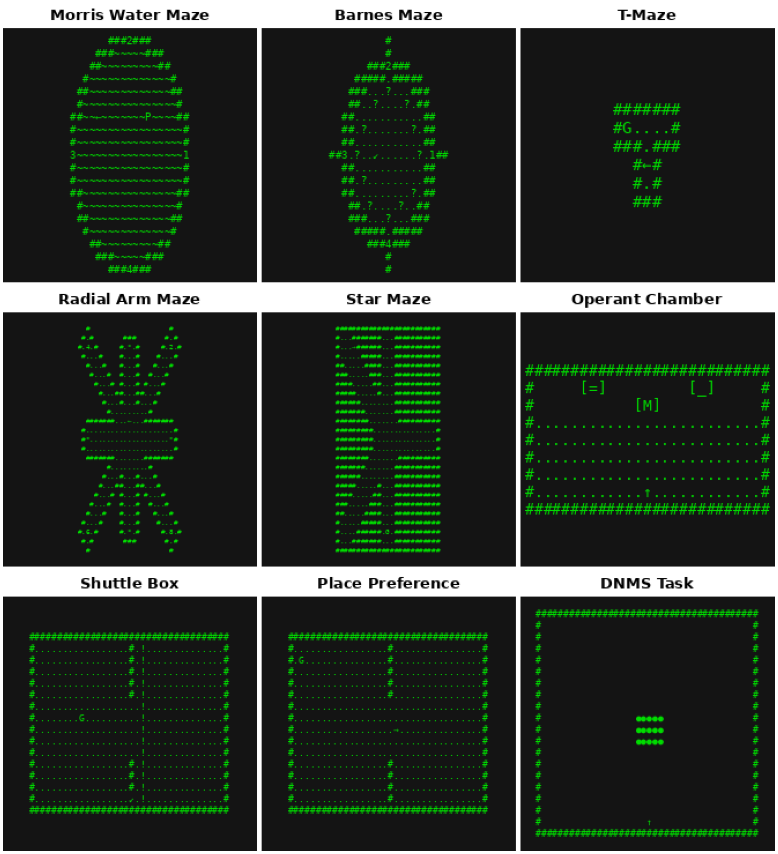
\includegraphics[width=\columnwidth]{fig_environments.pdf}
\caption{ASCII renderings of all nine CheeseBench environments as seen by the model. Walls are shown as \texttt{\#}, traversable areas as \texttt{\~{}} or \texttt{.}, goals as \texttt{G}, and the agent arrow indicates position and facing direction.}
\label{fig:environments}
\end{figure}

\begin{table}[t]
\centering
\caption{CheeseBench environments. Animal baselines are from published rodent studies. Trials = evaluation trials; Steps = max steps/trial.}
\label{tab:environments}
\resizebox{\columnwidth}{!}{%
\begin{tabular}{@{}llcrr@{}}
\toprule
Environment & Cognitive Dimension & Species & Trials & Steps \\
\midrule
MorrisWaterMaze & Spatial Learning & C57BL/6 & 20 & 500 \\
BarnesMaze & Spatial Learning & C57BL/6 & 16 & 300 \\
StarMaze & Spatial Learning & C57BL/6 & 40 & 300 \\
TMaze & Ego. Navigation & NMRI & 40 & 200 \\
RadialArmMaze & Working Memory & C57BL/6 & 20 & 400 \\
DNMSTask & Working Memory & Long-Evans & 100 & 50 \\
OperantChamber & Instr. Conditioning & C57BL/6 & 50 & 100 \\
ShuttleBox & Avoidance Learning & SD rat & 40 & 50 \\
PlacePreference & Assoc. Learning & C57BL/6 & 12 & 300 \\
\bottomrule
\end{tabular}%
}
\end{table}


\subsection{Observation and Action Space}

Environments are rendered as ASCII text in three view modes (\Cref{fig:viewmodes}): \texttt{ASCII\_2D} (top-down bird's-eye map showing the full layout), \texttt{ASCII\_2D\_FPV} (egocentric cropped view centered on the agent), and \texttt{ASCII\_3D} (pseudo-3D first-person perspective using block shading).
The default mode used in all experiments is \texttt{ASCII\_2D}.
The action space consists of four egocentric actions: \texttt{FORWARD}, \texttt{ROTATE\_LEFT}, \texttt{ROTATE\_RIGHT}, and \texttt{STAY}.
At each turn, the agent produces up to $k$ actions and a free-text ``learnings'' field for explicit working memory, capped at 500 characters.

\begin{figure}[t]
\centering
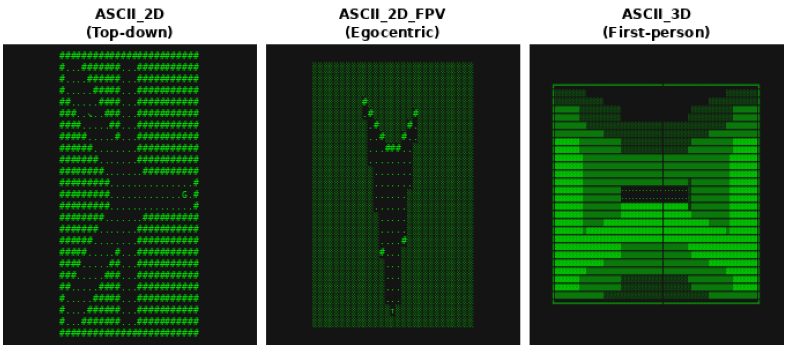
\includegraphics[width=\columnwidth]{fig_viewmodes.pdf}
\caption{The three ASCII observation modes for the Star Maze. \texttt{ASCII\_2D} provides a full top-down text map; \texttt{ASCII\_2D\_FPV} shows an egocentric cropped view centered on the agent; \texttt{ASCII\_3D} renders a pseudo-3D first-person perspective with depth shading.}
\label{fig:viewmodes}
\end{figure}

\subsection{System Prompt}

The unified system prompt describes the action space and output format but provides \emph{no} information about task goals, reward structure, or environment layout.
It also includes generic strategy guidance (attend to reward signals, track spatial position, form and test hypotheses, plan efficiently), which is identical across all tasks:

\begin{quote}
\itshape
``You are an embodied agent placed in a behavioral experiment. Your only goal is to maximize cumulative reward. [\ldots] STRATEGY: 1.~Reward signals: positive $\to$ repeat, negative $\to$ change. 2.~Spatial memory: track position. 3.~Hypothesis testing. 4.~Pattern recognition. 5.~Efficient planning. [\ldots] Respond with LEARNINGS and up to $k$ ACTIONS.''
\end{quote}


\section{Experimental Setup}

\paragraph{Models.}
We evaluate six open-weight models from three families: \textbf{Qwen2.5-VL} at 3B, 7B, 32B, and 72B parameters \citep{bai2025qwen25}, \textbf{InternVL2.5-8B} \citep{chen2024internvl}, and \textbf{Phi-4-Multimodal-14B} \citep{abdin2024phi4}.
All models are served via vLLM on 8$\times$H100 80GB GPUs.
Although these are vision-language models by architecture, the main experiments use \texttt{ASCII\_2D} rendering, so the models receive only text input.

\paragraph{Protocol.}
Each model runs all 9 environments using the \texttt{ASCII\_2D} (text) view mode with default settings: history length $h{=}5$ observation-action pairs, action batch size $k{=}8$, default prompt variant.
The environment state is rendered as an ASCII character grid and sent as a text message; no images are involved.
We compare against two non-LLM baselines: a uniformly random agent and Tabular-QL, a reinforcement learning agent that hashes observations into discrete states, learns via tabular Q-learning, and builds a transition graph for BFS planning to previously discovered goals.
We also test a BFS oracle that parses the ASCII grid and navigates to any visible goal marker; this agent reaches 100\% success on tasks where the goal is visible in the grid (e.g., Morris Water Maze, where the hidden platform is rendered as a symbol visible to any text parser but requires spatial learning for the LLM agent to exploit).
We report success rates across all trials per environment; error bars in \Cref{fig:main_results} show binomial standard errors computed from the per-environment trial counts in \Cref{tab:environments} (12--100 trials depending on the task).
All runs use temperature~0.7 sampling with fixed environment seeds; stochastic environment dynamics and sampling are the sources of run-to-run randomness.
Each model--environment condition is a single run; we do not average over multiple seeds, so per-environment estimates carry non-trivial sampling uncertainty.
The approximate rodent values shown as diamond markers in figures are not measured in our environments; they are reference anchors derived from published learning curves under different protocols and outcome metrics (see the Rodent Baseline Construction appendix).

\paragraph{Ablations.}
Using Qwen2.5-VL-7B as the reference model, we ablate:
\begin{itemize}
    \item \textbf{History length} $h \in \{1, 3, 5, 10\}$: number of past observation-action pairs retained in context.
    \item \textbf{Prompt variant}: default, minimal (stripped-down), chain-of-thought (CoT), and few-shot (with example trajectories).
    \item \textbf{Action batch size} $k \in \{1, 4, 8, 16\}$: number of actions per API call.
    \item \textbf{Vision}: VLM with image input vs.\ text-only LLM (Qwen2.5-Instruct without vision encoder) at 7B and 32B scales, both using ASCII text observations. This tests whether the vision encoder helps even when the input is text.
\end{itemize}


\section{Results}

\subsection{Multi-Model Comparison}

\Cref{fig:main_results} shows per-environment success rates for all six models on ASCII text input.
The best overall model is Qwen2.5-VL-7B (52.6\%), followed by Qwen2.5-VL-72B (49.3\%) and Qwen2.5-VL-32B (48.0\%).
The random baseline averages 32.1\% and the Tabular-QL agent averages 31.2\%, but they succeed on very different tasks: Tabular-QL reaches 98\% on OperantChamber and 100\% on ShuttleBox through Q-learning, while scoring 0\% on all spatial environments.
All agents, including LLMs, fall well below the approximate rodent reference values (70--90\%), shown as diamond markers.

Performance varies widely across environments.
On \textbf{OperantChamber} (instrumental conditioning), Qwen2.5-VL-72B reaches 94.0\%, approaching the approximate rodent reference value, which suggests that simple stimulus-response associations are within reach of in-context learning.
On \textbf{ShuttleBox}, Qwen2.5-VL-32B reaches 95.0\%.
But \textbf{RadialArmMaze} (working memory) is nearly unsolved: the best model manages 5.0\%, compared to 70\% for rodents.
This task requires keeping track of which arms have been visited across 20+ steps within a single trial, which is very difficult for autoregressive models.

\begin{figure}[t]
\centering
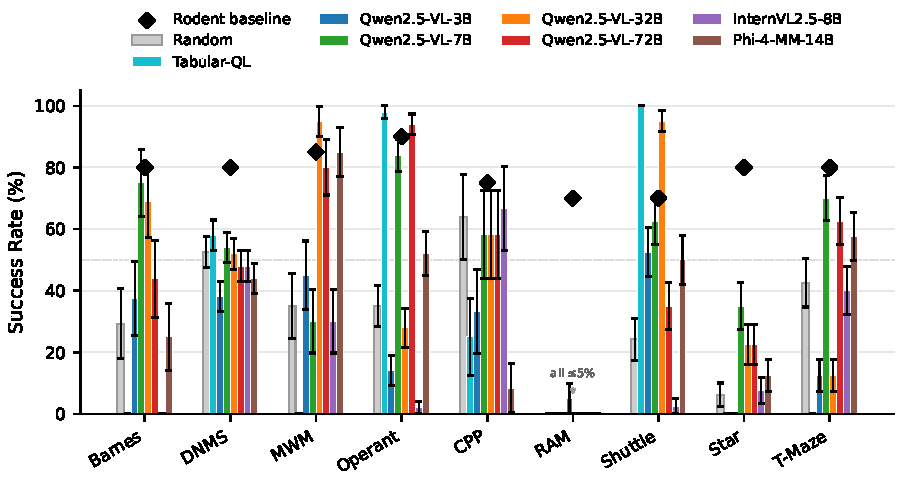
\includegraphics[width=\columnwidth]{fig_main_results.pdf}
\caption{Per-environment success rates (ASCII text input) for six LLMs, Tabular-QL, and random baseline compared to approximate rodent reference values (diamonds). The Radial Arm Maze remains essentially unsolved by all agents.}
\label{fig:main_results}
\end{figure}


\subsection{Cognitive Profile}

\Cref{fig:radar} shows the cognitive profile of the largest Qwen model (Qwen2.5-VL-72B) compared to rodent reference values, as it displays the clearest contrast across cognitive dimensions.
It reaches 94\% on instrumental conditioning, where simple reward associations suffice, but drops to 24\% on working memory (vs.\ 75\% for rodents).
Spatial learning (49\% vs.\ 82\%) and avoidance learning (35\% vs.\ 70\%) fall in between.
The pattern suggests that LLMs can learn reactive associations through in-context learning but struggle with tasks requiring sustained state tracking.

\begin{figure}[t]
\centering
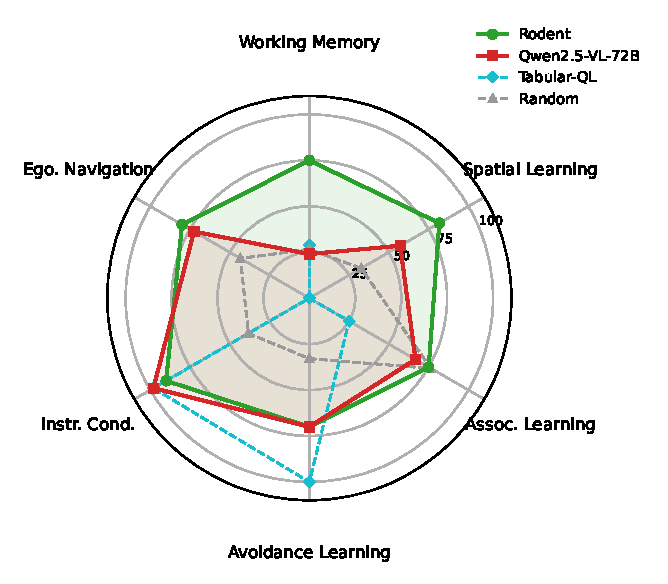
\includegraphics[width=0.75\columnwidth]{fig_cognitive_radar.pdf}
\caption{Cognitive profile across six dimensions. The LLM and Tabular-QL agent show complementary strengths: the LLM handles a broader range of tasks while Tabular-QL excels at conditioning through direct reinforcement learning.}
\label{fig:radar}
\end{figure}


\subsection{Scaling Behavior}

\Cref{fig:scaling} shows overall success rate vs.\ model size within the Qwen2.5-VL family.
There is a large jump from 3B (25.9\%) to 7B (52.6\%), but performance plateaus beyond 7B, with 32B (48.0\%) and 72B (49.3\%) performing similarly; the differences among the 7B, 32B, and 72B models are within binomial standard error and thus not statistically significant.
This saturation contrasts with typical benchmark scaling laws.
InternVL2.5-8B (21.9\%) and Phi-4-MM-14B (37.1\%) underperform the comparable-sized Qwen models, so model family and training data clearly matter too.

\begin{figure}[t]
\centering
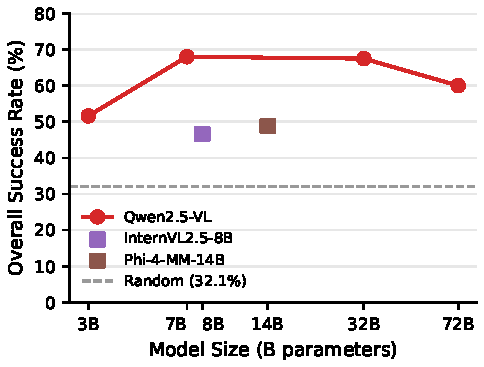
\includegraphics[width=0.75\columnwidth]{fig_scaling.pdf}
\caption{Scaling behavior: performance saturates beyond 7B under this protocol.}
\label{fig:scaling}
\end{figure}


\subsection{Ablation Studies}

\Cref{fig:ablations} summarizes the four ablation dimensions.

\emph{Note on ablation protocol:} to manage compute, ablation runs use a flat 15 trials per environment rather than the per-environment protocol in \Cref{tab:environments}, and each condition is a separate run.
With only 15 trials, per-condition estimates carry substantial sampling noise (binomial 95\% CI of $\pm$25pp at $p{=}0.5$), so the ``default'' ablation baseline ($h{=}5$, $k{=}8$, default prompt) need not exactly match the 52.6\% multi-model result for the same model.
Trends should be interpreted directionally; individual effect sizes are approximate.

\paragraph{History length (\Cref{fig:ablations}a).}
Shorter history tends to give better results: $h{=}1$ achieves 57.0\% vs.\ 26.7\% for $h{=}10$, though with 15 trials per environment the absolute values are noisy (see protocol note above).
The directional trend is consistent with the model having trouble picking out relevant past observations from longer context.
With $h{=}1$, the ``learnings'' field (500 characters of free-text working memory) becomes the only long-term memory, and the model appears to use it more effectively.

\paragraph{Prompt strategy (\Cref{fig:ablations}b).}
The default prompt (46.7\%) outperforms chain-of-thought (31.9\%), minimal (35.6\%), and few-shot (29.6\%).
CoT hurting is worth noting: step-by-step reasoning appears to waste context tokens on verbose output that displaces useful observation history.
Few-shot examples may bias the model toward mimicking the demonstrated trajectories instead of adapting to new environments.

\paragraph{Action batch size (\Cref{fig:ablations}c).}
Performance is highest at $k{=}4$ (51.9\%), followed by $k{=}8$ (45.9\%), with poor results at the extremes, $k{=}1$ (28.9\%) and $k{=}16$ (20.0\%).
With $k{=}1$, the API call overhead means fewer observations per episode.
With $k{=}16$, the model must plan 16 steps ahead without feedback, which is too long for reliable open-loop control.

\paragraph{Vision vs.\ text-only (\Cref{fig:ablations}d).}
This ablation compares VLM architectures (with vision encoder) against text-only LLMs (without vision encoder), both receiving ASCII text.
At 7B, the VLM (41.5\%) outperforms text-only (21.5\%) by 20 percentage points.
While this gap is consistent with the vision encoder providing an advantage even on text input, we cannot rule out alternative explanations such as differences in training data or fine-tuning procedures between the VLM and text-only variants.
At 32B, the pattern reverses: the VLM (32.6\%) underperforms text-only (43.0\%) by 10.4 percentage points, suggesting that at larger scales the vision encoder may interfere with text-based reasoning rather than help.

\begin{figure}[t]
\centering
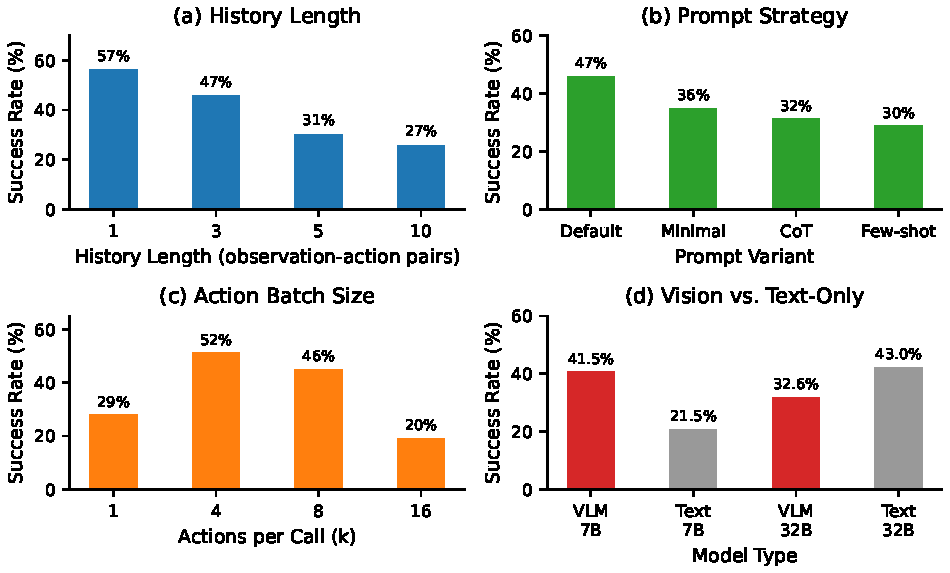
\includegraphics[width=\columnwidth]{fig_ablations.pdf}
\caption{Ablation studies (all on ASCII text input) using Qwen2.5-VL-7B (32B for vision ablation). (a)~Shorter history is better. (b)~Default prompt beats CoT. (c)~$k{=}4$ is the sweet spot. (d)~Vision encoder helps at 7B but hurts at 32B.}
\label{fig:ablations}
\end{figure}


\subsection{Image-Based Rendering}

We also tested pixel-based rendering (\texttt{TOPDOWN\_2D}) but found the renderer produced low-quality images.
Results from this mode are therefore not reported here; we focus on ASCII text input throughout.

\begin{table}[t]
\centering
\caption{Summary of main results and ablations. All values are overall success rates (\%) on ASCII text input. Multi-model uses per-environment trial counts (\Cref{tab:environments}); ablations use 15~trials/env in separate runs and thus may differ from multi-model values for the same configuration.}
\label{tab:summary}
\resizebox{\columnwidth}{!}{%
\begin{tabular}{@{}lr@{\hspace{12pt}}lr@{}}
\toprule
\textbf{Multi-model} & \textbf{\%} & \textbf{Ablation} & \textbf{\%} \\
\midrule
Qwen2.5-VL-7B  & 52.6 & History $h{=}1$   & 57.0 \\
Qwen2.5-VL-72B & 49.3 & History $h{=}3$   & 46.7 \\
Qwen2.5-VL-32B & 48.0 & History $h{=}5$   & 31.1 \\
Phi-4-MM-14B   & 37.1 & History $h{=}10$  & 26.7 \\
Qwen2.5-VL-3B  & 25.9 & Actions $k{=}4$   & 51.9 \\
InternVL2.5-8B & 21.9 & Actions $k{=}8$   & 45.9 \\
\cmidrule(r){1-2}
Random         & 32.1 & Prompt: default    & 46.7 \\
Tabular-QL     & 31.2 & Prompt: CoT        & 31.9 \\
Rodent (approx.)& 78.9 & VLM-7B / Text-7B  & 41.5 / 21.5 \\
               &      & VLM-32B / Text-32B & 32.6 / 43.0 \\
\bottomrule
\end{tabular}%
}
\end{table}

\section{Discussion}

The results reveal a coherent pattern across all experiments.
We first summarize the empirical findings, then discuss possible interpretations.

\paragraph{Findings.}
(1)~Radial Arm Maze is nearly unsolved by all agents (0--5\%), while conditioning tasks approach or exceed rodent reference values.
(2)~Performance jumps from 3B to 7B but does not improve further at 32B or 72B.
(3)~Shorter history ($h{=}1$) outperforms longer history ($h{=}10$) by 30 percentage points, though ablation estimates are noisy (15 trials/env).
(4)~Chain-of-thought prompting hurts.
(5)~$k{=}4$ actions per call is the sweet spot; extreme values degrade performance.
These patterns are robust across models and are consistent with a profile in which LLM agents handle reactive associations but struggle with within-trial state tracking.

\paragraph{Interpretations.}
The findings are consistent with several possible explanations, which we present as hypotheses rather than conclusions.

\emph{State-tracking bottleneck.}
The near-total failure on RAM and the inverted history-length result both point toward difficulty maintaining and updating internal state representations.
In biological agents, hippocampal place cells and prefrontal working memory circuits support within-trial state tracking automatically.
In our LLM agents, the only state-tracking mechanism is the 500-character ``learnings'' scratchpad, updated only between API calls.
This is a hypothesis about the \emph{agent-plus-interface system}, not a claim about the transformer architecture in isolation: a different interface (e.g., per-step scratchpad updates, external memory, or fine-tuned policies) might substantially change the outcome.

\emph{Context management.}
The inverted history-length result ($h{=}1 > h{=}10$) suggests that the model cannot selectively attend to relevant past observations when mixed with stale ones.
With $h{=}1$, the learnings field becomes the sole persistent memory, and the model appears to use it more effectively as a compressed summary.
Again, this may reflect the specific prompting interface as much as an inherent limitation.

\emph{Scaling saturation.}
The plateau beyond 7B contrasts with typical NLP benchmark scaling.
One interpretation is that for procedural behavioral tasks, the bottleneck is not world knowledge or language understanding but the ability to plan under uncertainty given the information available in the prompt.
However, we cannot rule out that a different prompt design or training procedure could unlock further gains at larger scales.

\paragraph{Agent-Plus-Interface Evaluation.}
Since observed performance is tightly coupled to interface design (history length, action batching, scratchpad size, prompt variant), CheeseBench should be understood as evaluating the \emph{agent-plus-interface system}, not raw latent model cognition.
The ablation results demonstrate this clearly: the same model's performance ranges from 20\% to 57\% depending on interface parameters alone.
This framing does not weaken the benchmark; it sharpens the question from ``how smart is the model?'' to ``how well does this agent configuration perform on procedural discovery tasks?''

\paragraph{Limitations.}
The comparison between LLM and rodent performance is not fully symmetric: animal baselines are approximate values derived from published learning curves and represent asymptotic performance after multiple training sessions, while our LLM agents are evaluated zero-shot within a single benchmark run under a specific prompting protocol and interface.
The gap we report is therefore specific to this protocol; a different interface (e.g., longer scratchpad, per-step memory updates, or a fine-tuned policy) could narrow it.
The environments are simplified gridworlds that lack the sensory richness of real rodent arenas; we discuss what is preserved and what is lost in Appendix~A.
Additionally, in the Morris Water Maze implementation, the hidden platform is rendered as a visible symbol in the ASCII grid; the BFS oracle exploits this, and the 100\% BFS score on MWM reflects symbol-parsing ability rather than spatial search.
LLM agents also occasionally produce unparseable outputs (e.g., invalid action strings), which are counted as wasted steps; the rate varies across models (from near-zero for larger models to $\sim$0.5 per trial for 3B models) and represents a confound separate from cognitive ability.
We evaluate open-weight models only; proprietary models may perform differently.
We also do not test interventions (e.g., external memory, recurrence, or fine-tuning) that could directly probe hypothesized bottlenecks; such experiments are a natural next step.


\section{Conclusion}

Under a unified zero-shot ASCII protocol, current open-weight LLM agents remain well below approximate rodent reference values on standardized behavioral paradigms.
The benchmark exposes a structured pattern: LLM agents handle simple conditioning but struggle with spatial navigation and within-trial state tracking.
Because performance is tightly coupled to interface design, these results characterize the agent-plus-interface system rather than raw model cognition.
Nonetheless, the magnitude of the gap on spatial and memory tasks is substantial and persists across model scales, suggesting that closing it will require targeted interventions beyond scaling alone.
We hope this work encourages the Artificial Life community to explore memory-augmented agent architectures and to use behavioral neuroscience as a grounding discipline for evaluating artificial cognition.

The benchmark code and all experimental results will be publicly released upon publication.


\bibliographystyle{apalike}
\bibliography{references}


\appendix
\section{Environment Fidelity}
\label{app:fidelity}

\Cref{tab:fidelity} summarizes what each CheeseBench environment preserves from the original rodent protocol and what is simplified.
The core simplification shared by all tasks is the reduction to a discrete gridworld with four egocentric actions and ASCII text rendering.
Despite these abstractions, each environment retains the essential cognitive demand of the source paradigm: spatial navigation tasks still require allocentric or egocentric mapping, working memory tasks still require tracking visited locations across steps, and conditioning tasks still require associating stimuli with rewards or punishments from scalar feedback alone.

\begin{table*}[t]
\centering
\caption{Environment fidelity summary. \textbf{P}: preserved from rodent protocol. \textbf{S}: simplified away. \textbf{C}: cognitive demand retained.}
\label{tab:fidelity}
\footnotesize
\begin{tabular}{@{}lp{14cm}@{}}
\toprule
\textbf{Environment} & \textbf{P / S / C} \\
\midrule
MWM & \textbf{P:} Hidden goal, distal landmarks, multiple starts. \textbf{S:} Continuous swim $\to$ grid; no currents. \textbf{C:} Allocentric spatial learning. \\[3pt]
Barnes & \textbf{P:} Escape hole among decoys, aversive motivation. \textbf{S:} Light/noise $\to$ step penalty; 3D $\to$ 2D. \textbf{C:} Spatial reference memory. \\[3pt]
Star & \textbf{P:} Radial corridors, strategy choice. \textbf{S:} Hidden goal $\to$ visible marker; continuous motion $\to$ grid; corridor width. \textbf{C:} Spatial strategy selection. \\[3pt]
T-Maze & \textbf{P:} T-corridor, forced choice, reward at one arm. \textbf{S:} Olfactory/tactile cues; continuous turning. \textbf{C:} Egocentric navigation. \\[3pt]
RAM & \textbf{P:} 8 arms (4 baited), revisit tracking. \textbf{S:} Odor trails; arm length variation; no explicit revisit penalty. \textbf{C:} Working memory across choices. \\[3pt]
DNMS & \textbf{P:} Sample--delay--choice, non-match rule. \textbf{S:} Object features $\to$ symbols; step-based delay. \textbf{C:} Working memory + rule learning. \\[3pt]
Operant & \textbf{P:} Levers, magazine, free-operant schedule. \textbf{S:} Pellet $\to$ scalar reward; no hunger drive. \textbf{C:} Instrumental conditioning. \\[3pt]
Shuttle & \textbf{P:} Two compartments, CS$\to$US, avoidance. \textbf{S:} Auditory CS $\to$ text; shock $\to$ neg.\ reward. \textbf{C:} Avoidance learning. \\[3pt]
CPP & \textbf{P:} Two chambers, one reward-paired, preference test. \textbf{S:} Drug/food $\to$ reward signal; floor $\to$ ASCII. \textbf{C:} Associative place learning. \\
\bottomrule
\end{tabular}
\end{table*}

\section{Rodent Baseline Construction}
\label{app:baselines}

\Cref{tab:baselines} documents how each approximate rodent baseline was derived.
Baselines are not single numbers extracted from one paper; they are approximate asymptotic success rates estimated from published learning curves for the relevant paradigm and species.
We mapped each paradigm's standard outcome metric (escape latency, error count, lever-press rate, etc.) to a binary success criterion appropriate for the gridworld implementation, then estimated the proportion of trials meeting that criterion at the end of training based on the shape of published learning curves.
These values should be treated as order-of-magnitude reference points, not precise quantitative benchmarks.

\begin{table*}[t]
\centering
\caption{Rodent baseline construction. Approx.\ = approximate asymptotic success rate used in figures. Sessions = number of training sessions modeled in the learning curve. PMC = PubMed Central source article for protocol.}
\label{tab:baselines}
\footnotesize
\begin{tabular}{@{}lcclp{10cm}@{}}
\toprule
\textbf{Env} & \textbf{Approx.} & \textbf{Sess.} & \textbf{PMC} & \textbf{Notes} \\
\midrule
MWM & 85\% & 5 & PMC3259155 & Platform acquisition, C57BL/6 mice, 5 trials/sess. Metric is path length; mapped to binary (reach platform within step limit). \\[2pt]
Barnes & 80\% & 5 & PMC1783636 & 12 holes, 4 trials/sess. Metric: primary errors $\to$ binary correct-hole. \\[2pt]
Star & 80\% & 10 & PMC3695082 & 5-arm maze, 4 trials/sess. Metric: reach goal arm via correct path. \\[2pt]
T-Maze & 80\% & 4 & PMC3399492 & Forced alternation, 10 trials/sess. Metric: correct arm on free choice. \\[2pt]
RAM & 70\% & 6 & PMC4030456 & 8 arms, 4 baited. Collect all rewards with 0 WM errors. Conservative; original rats scored higher on simpler metrics. \\[2pt]
DNMS & 80\% & 30 & PMC3982138 & Touchscreen TUNL task (rats). Criterion is 80\% correct on large separations at short delay. \\[2pt]
Operant & 90\% & 5 & PMC6619163 & FR-1 schedule, C57BL/6 mice, 20-min sess. Metric: lever press within step limit. Value reflects post-criterion steady-state performance; mean sessions to criterion is 6.5. \\[2pt]
Shuttle & 70\% & 5 & PMC4633642 & Active avoidance, Sprague-Dawley rats, 30 trials/sess. Metric: shuttle before US onset. Value from exercised group; sedentary controls reach $\sim$53\%. \\[2pt]
CPP & 75\% & 6 & PMC6101638 & 3-phase protocol. Metric: $>$55\% time in reward-paired chamber. \\
\bottomrule
\end{tabular}
\end{table*}

\end{document}
